\chapter{随机变量及其分布}

\intro{
	引入随机变量的概念，将样本空间中的结果映射到实数集，使概率论可以与微积分等分析工具结合。
}

\section{随机变量的概念}

\begin{mydefinition}{随机变量}
	设 $S = \{e\}$ 是试验的样本空间，如果量 $X$ 是定义在 $S$ 上的一个单值实值函数，即
	\[X: S \to \R,\]
	则称 $X$ 为\textbf{随机变量}（r.v.）。
\end{mydefinition}

随机变量的引入意义在于将随机试验的结果数量化，从而可以用数学分析的方法来研究随机现象。

\textbf{分类：}
\begin{itemize}
	\item \textbf{离散型随机变量：} 取值有限或可列无穷多个；
	\item \textbf{连续型随机变量：} 取值充满某个区间，分布函数可表为密度函数的积分；
	\item \textbf{奇异型/混合型：} 非以上二者。
\end{itemize}

\section{离散型随机变量的分布律}

\begin{mydefinition}{分布律（概率质量函数，PMF）}
	若 $X$ 取值 $x_1, x_2, \ldots, x_k, \ldots$ 且取这些值的概率依次为 $p_1, p_2, \ldots, p_k, \ldots$，则称
	\[P\{X = x_k\} = p_k\quad (k = 1, 2, \ldots)\]
	为 $X$ 的\textbf{分布律}。
\end{mydefinition}

\begin{myproperty}{分布律的基本性质}
\begin{enumerate}
	\item 非负性：$p_k \geq 0$；
	\item 归一性：$\displaystyle\sum_{k} p_k = 1$。
\end{enumerate}
\end{myproperty}

\subsection{常见的离散型分布}

\begin{myTheorem}{两点分布（0-1分布）}
记作 $X \sim B(1,p)$。用于描述一次 Bernoulli 试验（只有成功和失败两种结果）。
\begin{center}
\begin{tabular}{c|cc}
\toprule
$X$   & $1$     & $0$   \\
\midrule
$p_k$ & $p$     & $1-p$ \\
\bottomrule
\end{tabular}
\end{center}
\end{myTheorem}

\begin{myTheorem}{二项分布}
记作 $X \sim B(n,p)$。$X$ 表示 $n$ 重 Bernoulli 试验中事件 $A$ 发生的次数，$p = P(A)$。
\begin{myformula}
\boxed{\displaystyle P\{X = k\} = C_n^k p^k (1-p)^{n-k},\quad k = 0, 1, 2, \ldots, n.}
\end{myformula}
\end{myTheorem}

\begin{figure}[htbp]
\centering
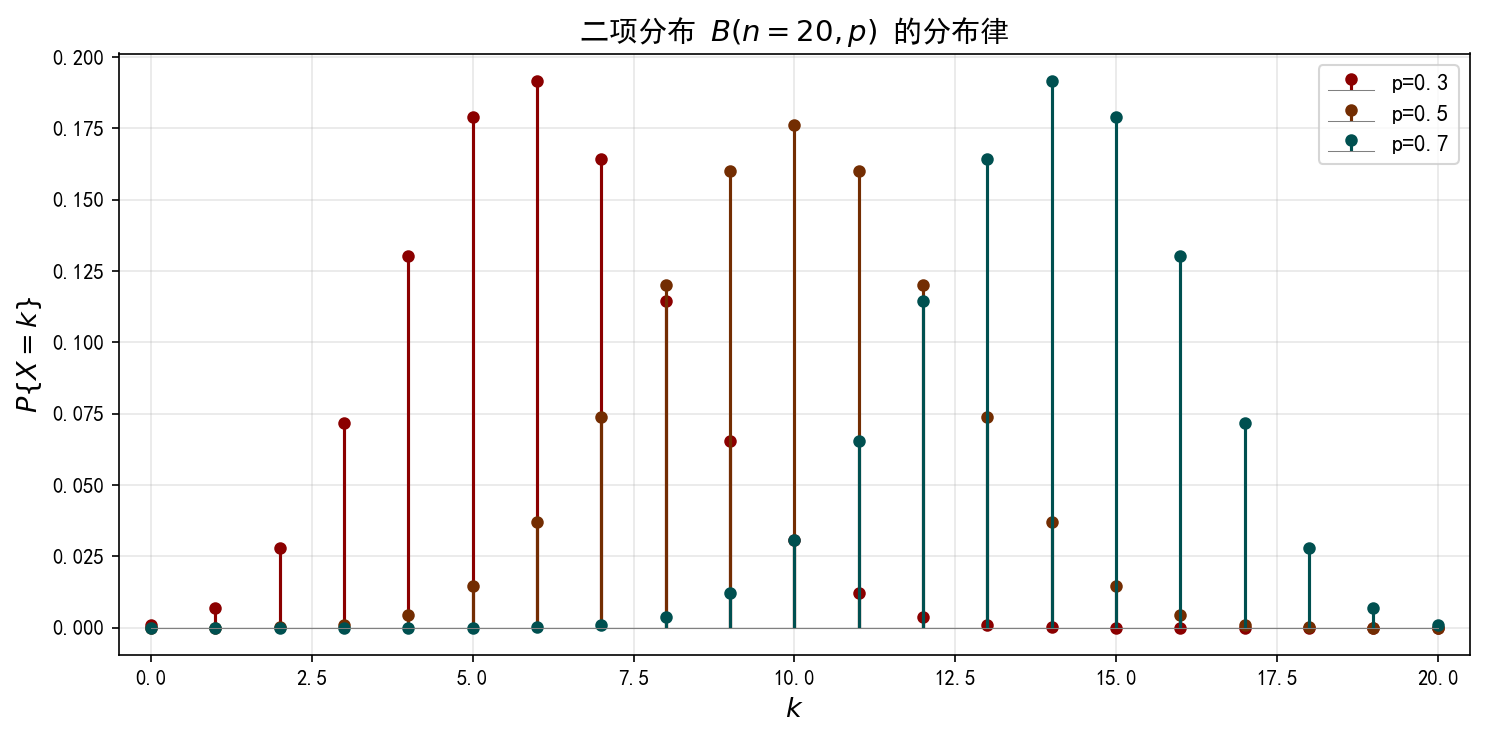
\includegraphics[width=0.85\textwidth]{Figure/binomial_dist.png}
\caption{二项分布 $B(20,p)$ 在不同 $p$ 下的分布律}
\end{figure}

\begin{myTheorem}{Poisson 分布 \,$X \sim P(\lambda)$}
参数 $\lambda > 0$ 表示单位时间内随机事件的平均发生次数。
\begin{myformula}
\boxed{\displaystyle P\{X = k\} = \frac{\lambda^k}{k!} e^{-\lambda},\quad k = 0, 1, 2, \ldots}
\end{myformula}
\end{myTheorem}

\begin{theorem}[Poisson 逼近定理]
当 $n$ 很大而 $p$ 很小时，二项分布 $B(n,p)$ 可用 Poisson 分布 $P(np)$ 近似：
\[C_n^k p^k (1-p)^{n-k} \approx \frac{(np)^k}{k!} e^{-np}.\]
一般当 $n \geq 20$，$p \leq 0.05$ 时，近似效果较好。
\end{theorem}

\begin{figure}[htbp]
\centering
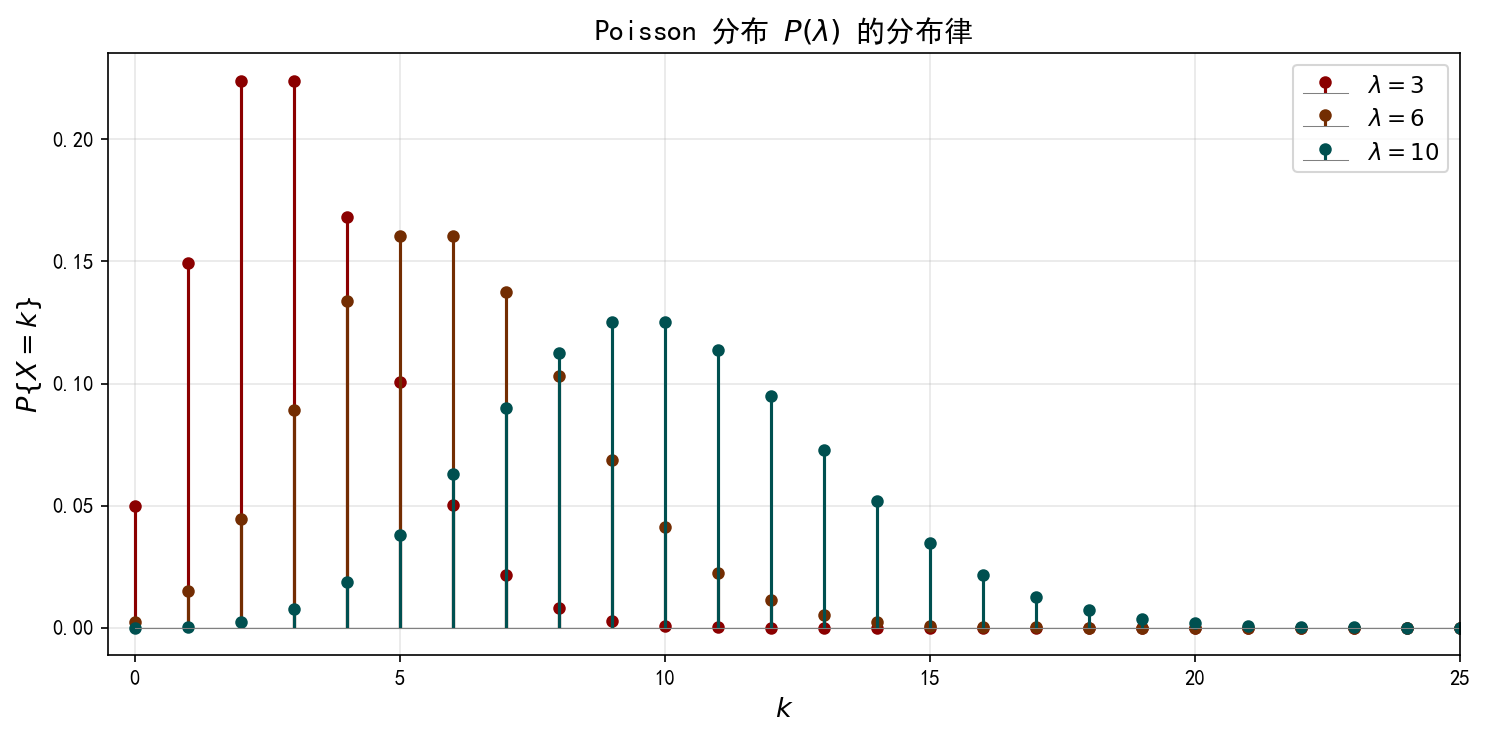
\includegraphics[width=0.85\textwidth]{Figure/poisson_dist.png}
\caption{Poisson 分布 $P(\lambda)$ 在不同参数 $\lambda$ 下的分布律}
\end{figure}

\begin{example}[Poisson 分布计算]
已知 $X \sim P(\lambda)$，且 $P\{X = 0\} = e^{-6}$，求 $P\{X \geq 2\}$。

\begin{solution}
由 $P\{X = 0\} = \frac{\lambda^0}{0!} e^{-\lambda} = e^{-\lambda} = e^{-6}$ 得 $\lambda = 6$。
\begin{align*}
P\{X \geq 2\} &= 1 - P\{X < 2\} \\
&= 1 - [P\{X = 0\} + P\{X = 1\}] \\
&= 1 - (e^{-6} + 6e^{-6}) = 1 - 7e^{-6} \approx 0.9826.
\end{align*}
\end{solution}
\end{example}

\section{随机变量的分布函数}

\begin{mydefinition}{分布函数（累积分布函数，CDF）}
	设 $X$ 是一个随机变量，\textbf{分布函数} $F(x)$ 定义为：
	\[F(x) = P\{X \leq x\},\quad -\infty < x < +\infty.\]
	由此可得：$P\{a < X \leq b\} = F(b) - F(a).$
\end{mydefinition}

\begin{myproperty}{分布函数的性质}
\begin{enumerate}
	\item \textbf{单调不减性：} 若 $x_1 < x_2$，则 $F(x_1) \leq F(x_2)$；
	\item \textbf{有界性：} $0 \leq F(x) \leq 1$，且
	\[\lim_{x \to -\infty} F(x) = 0,\quad \lim_{x \to +\infty} F(x) = 1;\]
	\item \textbf{右连续性：} $\displaystyle\lim_{x \to x_0^+} F(x) = F(x_0)$；
	\item 利用分布函数计算概率：
	\begin{align*}
		P\{a < X \leq b\} &= F(b) - F(a) \\
		P\{X > a\} &= 1 - F(a) \\
		P\{X = a\} &= F(a) - F(a-0) \\
		P\{X < a\} &= F(a-0)
	\end{align*}
\end{enumerate}
\end{myproperty}

\section{连续型随机变量及其概率密度}

\begin{mydefinition}{概率密度函数（PDF）}
	若存在非负函数 $f(x)$，使得 $X$ 的分布函数 $F(x)$ 可表示为
	\[F(x) = \int_{-\infty}^{x} f(t)\,dt,\]
	则称 $f(x)$ 为 $X$ 的\textbf{概率密度函数}，称 $X$ 为连续型随机变量。
\end{mydefinition}

\begin{myproperty}{概率密度函数的性质}
\begin{enumerate}
	\item 非负性：$f(x) \geq 0$；
	\item 归一性：$\displaystyle\int_{-\infty}^{+\infty} f(x)\,dx = 1$；
	\item 概率计算：$\displaystyle P\{a < X < b\} = \int_{a}^{b} f(x)\,dx = F(b) - F(a)$；
	\item 在 $f(x)$ 的连续点处：$F'(x) = f(x)$。
\end{enumerate}
\end{myproperty}

\subsection{常见的连续型分布}

\begin{myTheorem}{均匀分布}
记作 $X \sim U(a,b)$。
\begin{myformula}
\[f(x) = \begin{cases}
\dfrac{1}{b-a}, & a \leq x \leq b, \\[8pt]
0, & \text{其他}.
\end{cases}\qquad
F(x) = \begin{cases}
0, & x < a, \\[4pt]
\dfrac{x-a}{b-a}, & a \leq x < b, \\[8pt]
1, & x \geq b.
\end{cases}\]
\end{myformula}
\end{myTheorem}

\begin{figure}[htbp]
\centering
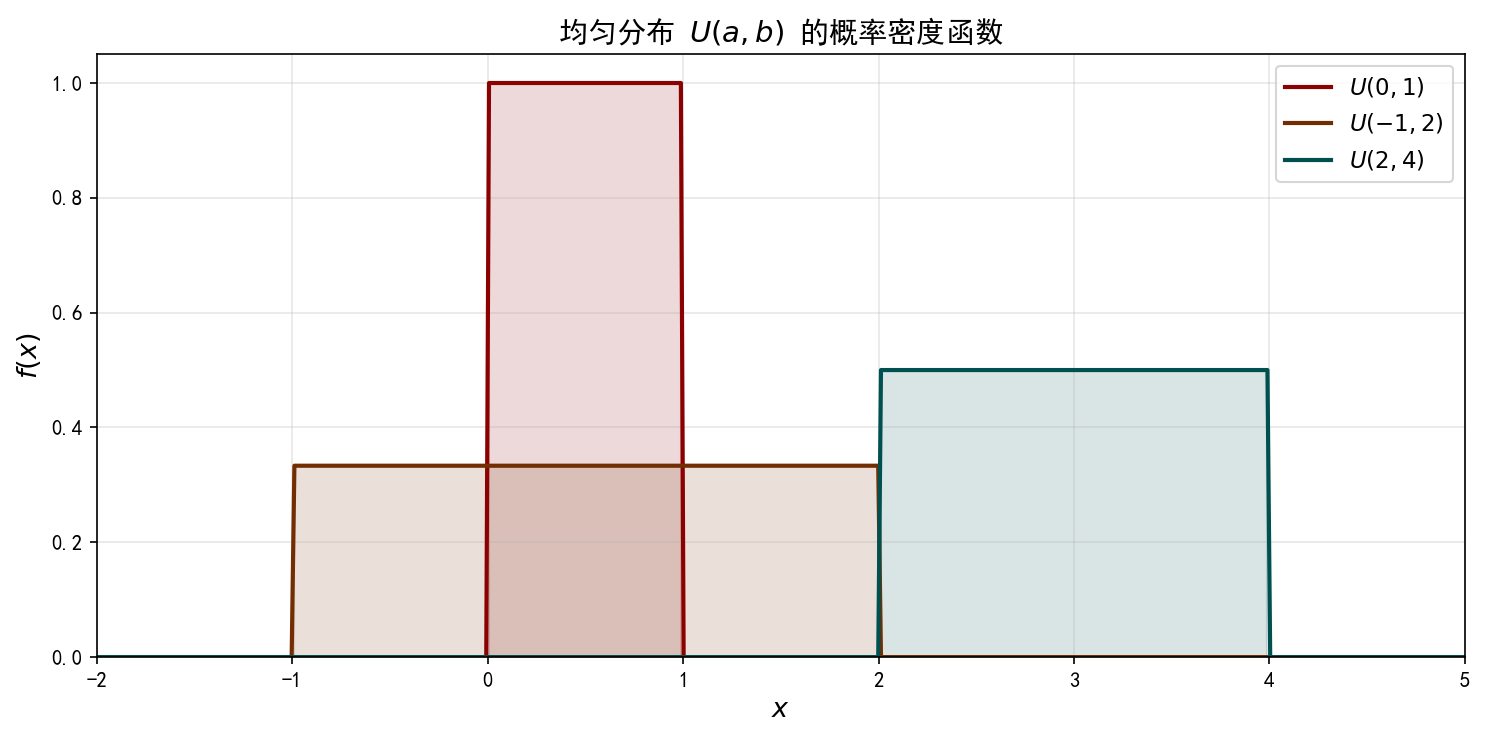
\includegraphics[width=0.85\textwidth]{Figure/uniform_dist.png}
\caption{均匀分布 $U(a,b)$ 的概率密度函数}
\end{figure}

\begin{myTheorem}{指数分布 \,$X \sim E(\lambda)$，$\lambda > 0$}
\begin{myformula}
\[f(x) = \begin{cases}
\lambda e^{-\lambda x}, & x \geq 0, \\
0, & x < 0.
\end{cases}\qquad
F(x) = \begin{cases}
1 - e^{-\lambda x}, & x \geq 0, \\
0, & x < 0.
\end{cases}\]
\end{myformula}
\end{myTheorem}

\begin{figure}[htbp]
\centering
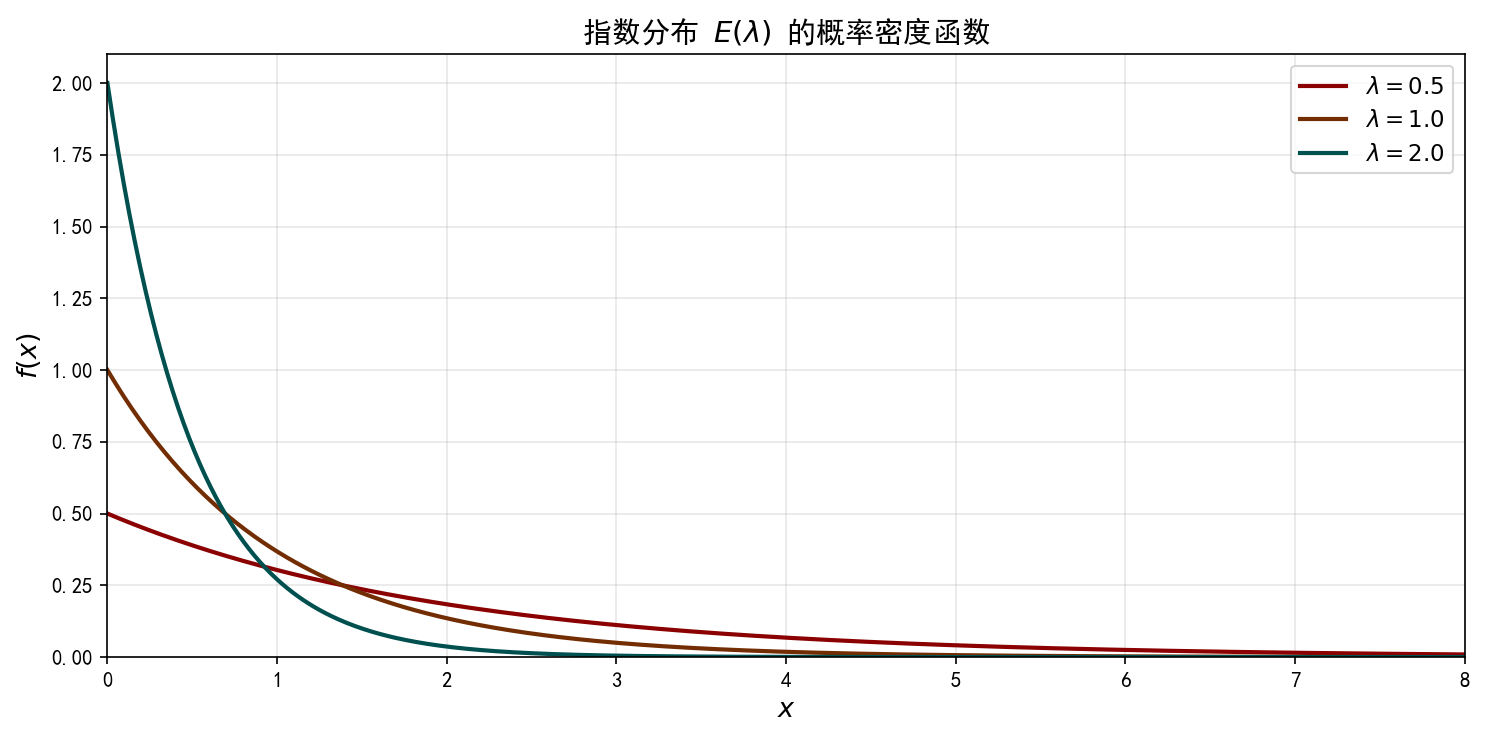
\includegraphics[width=0.85\textwidth]{Figure/exponential_dist.png}
\caption{指数分布 $E(\lambda)$ 在不同参数 $\lambda$ 下的概率密度函数}
\end{figure}

\begin{myTheorem}{指数分布的无记忆性}
对任意 $s, t > 0$，有
\[P(X > s + t \mid X > s) = P(X > t).\]
在连续型分布中，\textbf{只有指数分布具有无记忆性}。这意味着一个已经等待了 $s$ 时间的事件，继续等待 $t$ 时间的概率与从零开始等待 $t$ 时间的概率相同。

\textbf{证明：}
\begin{align*}
P(X > s + t \mid X > s) &= \frac{P(X > s + t,\, X > s)}{P(X > s)}
= \frac{P(X > s + t)}{P(X > s)} \\
&= \frac{1 - F(s+t)}{1 - F(s)} = \frac{e^{-\lambda(s+t)}}{e^{-\lambda s}} = e^{-\lambda t} = P(X > t).
\end{align*}
\end{myTheorem}

\begin{myTheorem}{正态（Gaussian）分布}
记作 $X \sim N(\mu, \sigma^2)$。
\begin{myformula}
\boxed{\displaystyle f(x) = \frac{1}{\sqrt{2\pi}\,\sigma} \exp\!\left(-\frac{(x-\mu)^2}{2\sigma^2}\right),\quad -\infty < x < +\infty.}
\end{myformula}
\end{myTheorem}

\textbf{标准正态分布} \,$Z \sim N(0, 1)$：
\begin{myformula}
\[\varphi(x) = \frac{1}{\sqrt{2\pi}} e^{-x^2/2},\qquad
\Phi(x) = \int_{-\infty}^{x} \varphi(t)\,dt.\]
\end{myformula}

\textbf{一般正态分布的标准化：}
\[Z = \frac{X - \mu}{\sigma} \sim N(0,1).\]

\begin{myTheorem}{$3\sigma$ 原则}
对于 $X \sim N(\mu, \sigma^2)$：
\begin{align*}
P\{\abs{X - \mu} < \sigma\} &\approx 0.6827, \\
P\{\abs{X - \mu} < 2\sigma\} &\approx 0.9545, \\
P\{\abs{X - \mu} < 3\sigma\} &\approx 0.9973.
\end{align*}
即正态随机变量取值几乎都落在均值 $\pm 3\sigma$ 的范围内。
\end{myTheorem}

\begin{figure}[htbp]
\centering
\begin{subfigure}{0.48\textwidth}
\centering
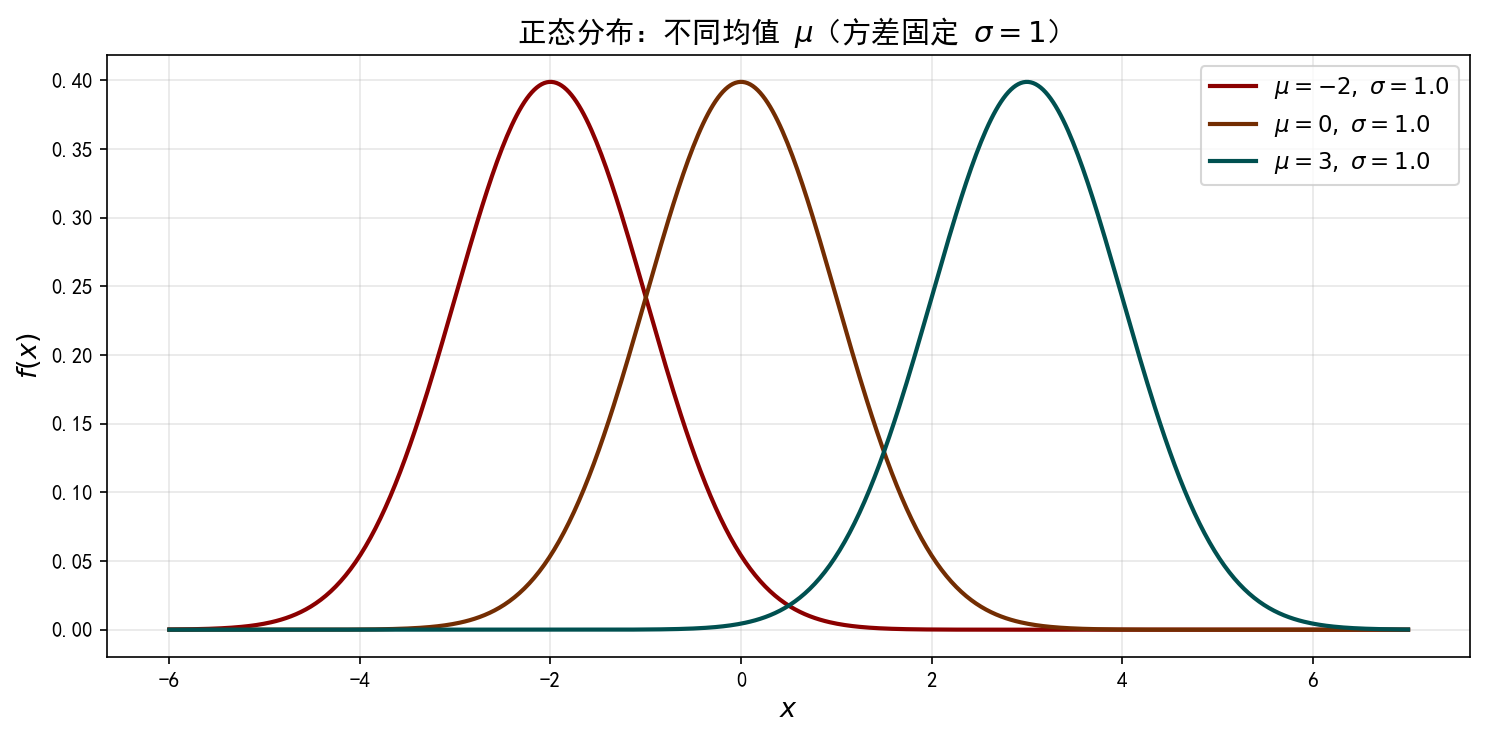
\includegraphics[width=\textwidth]{Figure/normal_mu.png}
\caption{不同 $\mu$，$\sigma=1$}
\end{subfigure}
\hfill
\begin{subfigure}{0.48\textwidth}
\centering
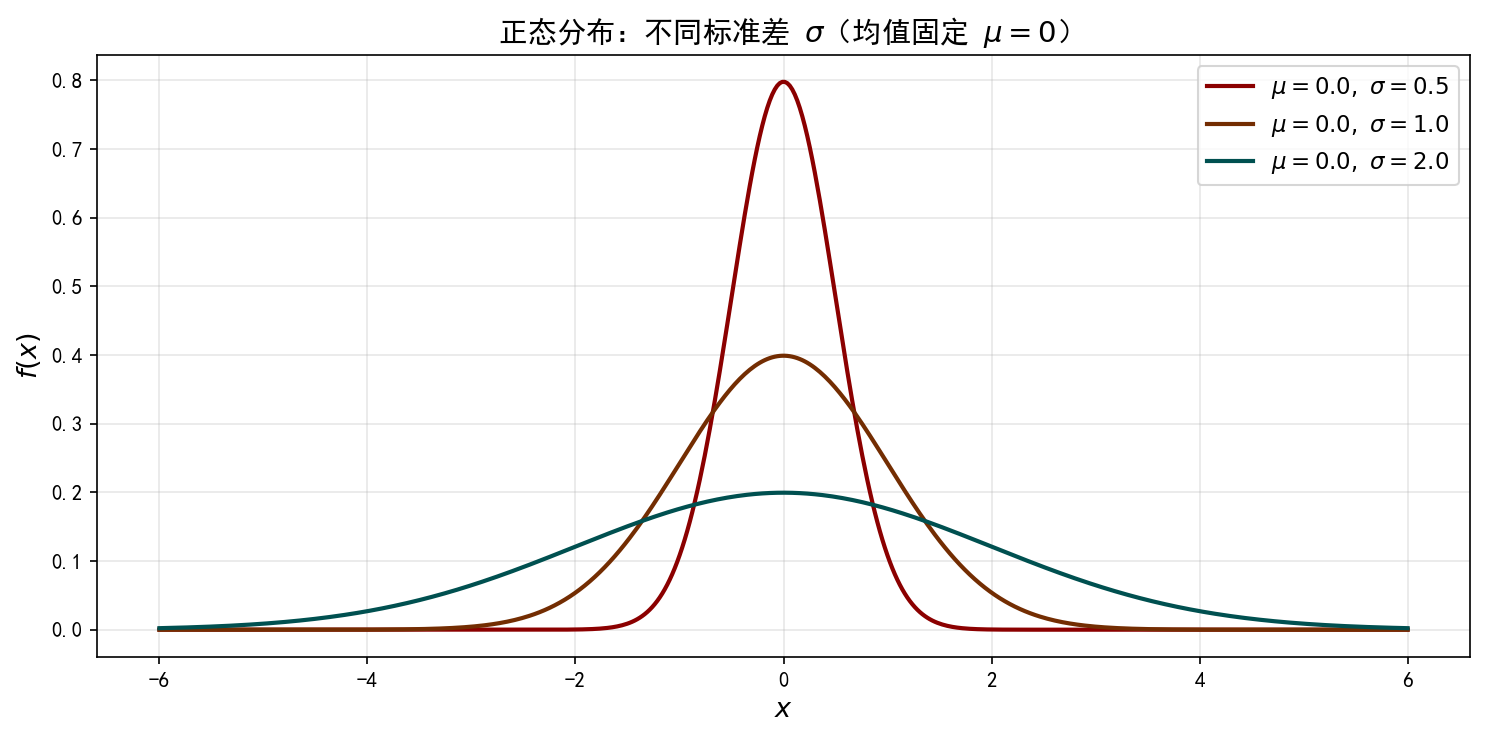
\includegraphics[width=\textwidth]{Figure/normal_sigma.png}
\caption{不同 $\sigma$，$\mu=0$}
\end{subfigure}
\caption{正态分布 $N(\mu,\sigma^2)$ 的概率密度函数}
\end{figure}

\begin{example}[求参数、概率与分布函数]
已知 $X$ 的概率密度函数为
\[f(x) = \begin{cases} A x^2, & 0 < x < 1, \\ 0, & \text{其他}. \end{cases}\]

\begin{solution}
\textbf{(1) 求参数 $A$：}
由归一性：
\[\int_{0}^{1} A x^2\,dx = A \cdot \frac{x^3}{3}\Big|_{0}^{1} = \frac{A}{3} = 1 \quad\Rightarrow\quad A = 3.\]

\textbf{(2) 求 $P\{0.5 < X < 3\}$：}
\[P\{0.5 < X < 3\} = \int_{0.5}^{1} 3x^2\,dx = x^3\Big|_{0.5}^{1} = 1 - 0.125 = 0.875.\]

\textbf{(3) 求分布函数 $F(x)$：}
\[F(x) = \begin{cases}
0, & x \leq 0, \\
\int_{0}^{x} 3t^2\,dt = x^3, & 0 < x < 1, \\
1, & x \geq 1.
\end{cases}\]
\end{solution}
\end{example}

\section{随机变量函数的分布}

\begin{theorem}[公式法（单调变换）]
设 $X \sim f_X(x)$，$Y = g(X)$ 是严格单调可导函数，$g^{-1}$ 为其反函数。则 $Y$ 的概率密度函数为：
\begin{myformula}
\boxed{\displaystyle f_Y(y) = f_X\bigl(g^{-1}(y)\bigr) \cdot \abs{\frac{d}{dy} g^{-1}(y)}.}
\end{myformula}
\end{theorem}

\begin{example}[线性变换]
已知 $X \sim N(\mu, \sigma^2)$，求 $Y = \dfrac{X - \mu}{\sigma}$ 的概率密度。

\begin{solution}
反函数 $x = g^{-1}(y) = \sigma y + \mu$，导数为 $\sigma$。故
\[f_Y(y) = f_X(\sigma y + \mu) \cdot \sigma = \frac{1}{\sqrt{2\pi}} e^{-y^2/2},\]
即 $Y \sim N(0, 1)$。
\end{solution}
\end{example}

\begin{remark}[非单调变换的处理]
若 $g$ 非单调，可先求分布函数再求导：
\[F_Y(y) = P\{g(X) \leq y\} = \int_{\{x: g(x) \leq y\}} f_X(x)\,dx,\]
然后 $f_Y(y) = F'_Y(y)$。
\end{remark}
